%
% ---------------------------------------------------------------
% Copyright (C) 2012-2018 Gang Li
% ---------------------------------------------------------------
%
% This work is the default powerdot-tuliplab style test file and may be
% distributed and/or modified under the conditions of the LaTeX Project Public
% License, either version 1.3 of this license or (at your option) any later
% version. The latest version of this license is in
% http://www.latex-project.org/lppl.txt and version 1.3 or later is part of all
% distributions of LaTeX version 2003/12/01 or later.
%
% This work has the LPPL maintenance status "maintained".
%
% This Current Maintainer of this work is Gang Li.
%
%

\documentclass[
 size=14pt,
 paper=smartboard,  %a4paper, smartboard, screen
 mode=present, 		%present, handout, print
 display=slides, 	% slidesnotes, notes, slides
 style=tuliplab,  	% TULIP Lab style
 pauseslide,
 fleqn,leqno]{powerdot}


\usepackage{cancel}
\usepackage{caption}
\usepackage{stackengine}
\usepackage{smartdiagram}
\usepackage{attrib}
\usepackage{amssymb}
\usepackage{amsmath} 
\usepackage{amsthm} 
\usepackage{mathtools}
\usepackage{rotating}
\usepackage{graphicx}
\usepackage{boxedminipage}
\usepackage{rotate}
\usepackage{calc}
\usepackage[absolute]{textpos}
\usepackage{psfrag,overpic}
\usepackage{fouriernc}
\usepackage{pstricks,pst-3d,pst-grad,pstricks-add,pst-text,pst-node,pst-tree}
\usepackage{moreverb,epsfig,subfigure}
\usepackage{color}
\usepackage{booktabs}
\usepackage{etex}
\usepackage{breqn}
\usepackage{multirow}
\usepackage{natbib}
\usepackage{bibentry}
\usepackage{gitinfo2}
\usepackage{siunitx}
\usepackage{nicefrac}
%\usepackage{geometry}
%\geometry{verbose,letterpaper}
\usepackage{media9}
\usepackage{animate}
%\usepackage{movie15}
\usepackage{auto-pst-pdf}

\usepackage{breakurl}
\usepackage{fontawesome}
\usepackage{xcolor}
\usepackage{multicol}



\usepackage{verbatim}
\usepackage[utf8]{inputenc}
\usepackage{/usr/local/texlive/dtk-logos}
\usepackage{tikz}
\usepackage{adigraph}
%\usepackage{tkz-graph}
\usepackage{hyperref}
%\usepackage{ulem}
\usepackage{pgfplots}
\usepackage{verbatim}
\usepackage{fontawesome}


\usepackage{todonotes}
% \usepackage{pst-rel-points}
\usepackage{animate}
\usepackage{fontawesome}

\usepackage{listings}
\lstset{frameround=fttt,
frame=trBL,
stringstyle=\ttfamily,
backgroundcolor=\color{yellow!20},
basicstyle=\footnotesize\ttfamily}
\lstnewenvironment{code}{
\lstset{frame=single,escapeinside=`',
backgroundcolor=\color{yellow!20},
basicstyle=\footnotesize\ttfamily}
}{}


\usepackage{hyperref}
\hypersetup{ % TODO: PDF meta Data
  pdftitle={Presentation Title},
  pdfauthor={Gang Li},
  pdfpagemode={FullScreen},
  pdfborder={0 0 0}
}


% \usepackage{auto-pst-pdf}
% package to show source code

\definecolor{LightGray}{rgb}{0.9,0.9,0.9}
\newlength{\pixel}\setlength\pixel{0.000714285714\slidewidth}
\setlength{\TPHorizModule}{\slidewidth}
\setlength{\TPVertModule}{\slideheight}
\newcommand\highlight[1]{\fbox{#1}}
\newcommand\icite[1]{{\footnotesize [#1]}}

\newcommand\twotonebox[2]{\fcolorbox{pdcolor2}{pdcolor2}
{#1\vphantom{#2}}\fcolorbox{pdcolor2}{white}{#2\vphantom{#1}}}
\newcommand\twotoneboxo[2]{\fcolorbox{pdcolor2}{pdcolor2}
{#1}\fcolorbox{pdcolor2}{white}{#2}}
\newcommand\vpspace[1]{\vphantom{\vspace{#1}}}
\newcommand\hpspace[1]{\hphantom{\hspace{#1}}}
\newcommand\COMMENT[1]{}

\newcommand\placepos[3]{\hbox to\z@{\kern#1
        \raisebox{-#2}[\z@][\z@]{#3}\hss}\ignorespaces}

\renewcommand{\baselinestretch}{1.2}


\newcommand{\draftnote}[3]{
	\todo[author=#2,color=#1!30,size=\footnotesize]{\textsf{#3}}	}
% TODO: add yourself here:
%
\newcommand{\gangli}[1]{\draftnote{blue}{GLi:}{#1}}
\newcommand{\shaoni}[1]{\draftnote{green}{sn:}{#1}}
\newcommand{\gliMarker}
	{\todo[author=GLi,size=\tiny,inline,color=blue!40]
	{Gang Li has worked up to here.}}
\newcommand{\snMarker}
	{\todo[author=Sn,size=\tiny,inline,color=green!40]
	{Shaoni has worked up to here.}}


%\input{../../../.git/gitHeadInfo.gin}

%%%%%%%%%%%%%%%%%%%%%%%%%%%%%%%%%%%%%%%%%%%%%%%%%%%%%%%%%%%%%%%%%%%%
% title
% TODO: Customize to your Own Title, Name, Address
%

\title{Credit Card Fraud Detection}
\author{
Lin Jiahong
\\
\\Nanjing University of Science and Technology
}
\date{\gitCommitterDate}


% Customize the setting of slides
\pdsetup{
% TODO: Customize the left footer, and right footer
rf=\href{http://www.tulip.org.au}{
Last Changed by: \textsc{\gitCommitterName}\ \gitVtagn-\gitAbbrevHash\ (\gitAuthorDate)
},
cf={Credit Card Fraud Detection},
}
\begin{document}

\maketitle

%\begin{slide}{Overview}
%\tableofcontents[content=sections]
%\end{slide}


%%==========================================================================================
%%
\begin{slide}[toc=,bm=]{Overview}
\tableofcontents[content=currentsection,type=1]
\end{slide}
%%
%%==========================================================================================


\section{Problem Definition}


%%==========================================================================================
%%
\begin{slide}{Credit Card Fraud Detection}
\begin{center}
\twotonebox{\rotatebox{90}{Defn}}{\parbox{.86\textwidth}
{Credit Card Fraud Detection aims to identify the presence of fraudulent credit card use through the characteristics of credit card use.
\begin{itemize}
\item Data covers   \textcolor{orange}{Preprocessing features} ,
 \textcolor{orange}{Time} and  \textcolor{orange}{Amount}.
\item The data comes with a label of behavior category.
\end{itemize}
}}

\end{center}
\begin{center}
	\begin{tabular}{c| c c c c c }
		\toprule
		%\centering
		Class & \texttt{row_num}  \\
		\midrule
		$All$
		&  {$284807$} \\
		$Normal$
		&  {$284315$} \\
		$Fraud$
		&  {$492$} \\
		\bottomrule
	\end{tabular}
\end{center}
%%============================================================================

\end{slide}
%%
%%==========================================================================================






\section{Data Analysis and Preprocessing}





%%==========================================================================================
%%
\begin{slide}[toc=,bm=]{Overall data}

\begin{itemize}
\item
Time- \textcolor{orange} {Transaction time of day in seconds.}
\end{itemize}

\begin{itemize}
	\item
	28 Features- \textcolor{orange} {['V1', 'V2', 'V3', 'V4', 'V5', 'V6', 'V7', 'V8', 'V9', 'V10', 'V11','V12', 'V13', 'V14', 'V15', 'V16', 'V17', 'V18', 'V19', 'V20', 'V21', 'V22', 'V23', 'V24', 'V25', 'V26', 'V27', 'V28']}
\end{itemize}

\begin{itemize}
	\item
	Amount - \textcolor{orange} {Real transaction amount}
\end{itemize}

\begin{itemize}
	\item
	Class - \textcolor{orange} {0 for normal behavior, 1 for abnormal behavior}
\end{itemize}

\begin{itemize}
	\item
	This anomaly detection task dataset is imbalanced datasets.
\end{itemize}


%%==========================================================================================


\end{slide}
%%
%%==========================================================================================


%%==========================================================================================
%%
\begin{slide}[toc=,bm=]{Amount and Time Distribution}
\begin{itemize}
	\item
	Fraud is smaller in amount and more evenly distributed over time.
\end{itemize}
\begin{figure}
  \centering
  \selectcolormodel{rgb}
  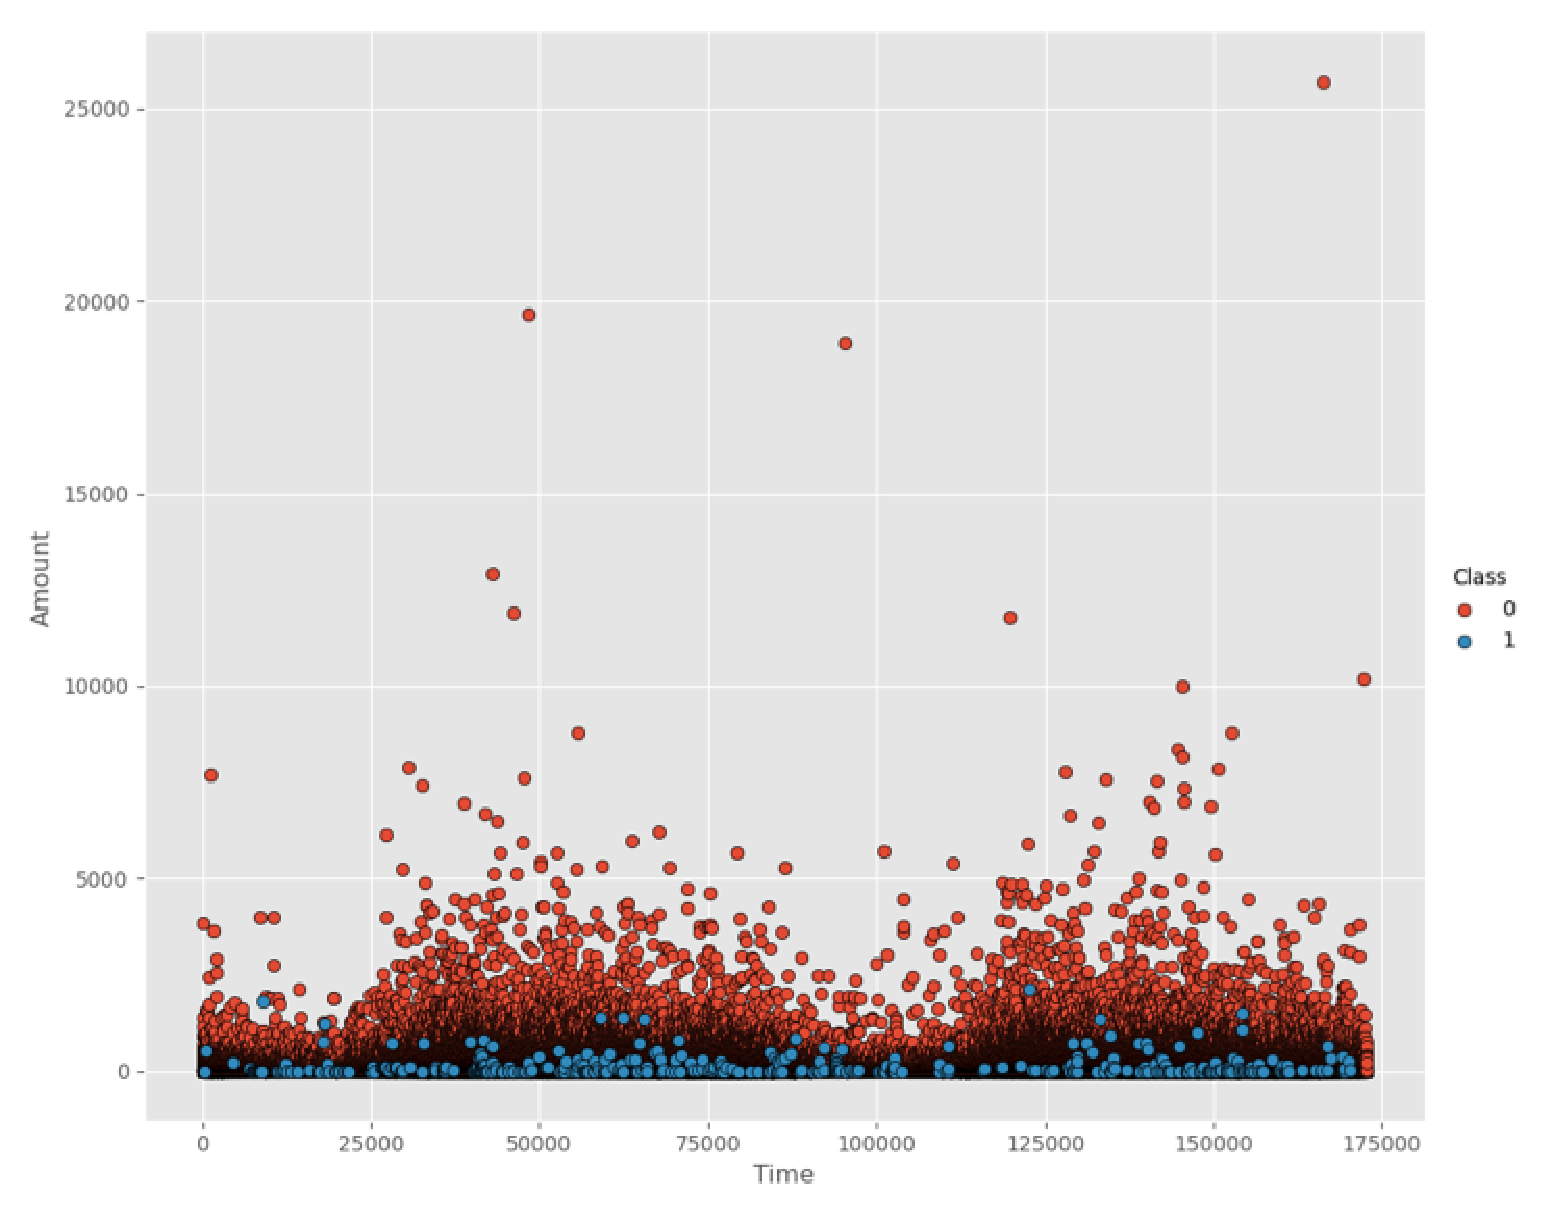
\includegraphics[scale=0.45]{amounttime.eps}
%  \includegraphics[width=0.5\textwidth]{figures//OutAspect_target.eps}\\
  \caption{Amount and Time Distribution Scatterplot}\label{fig:OutAspect-target}
\end{figure}
\end{slide}
%%
%%==========================================================================================


==============
%%
\begin{slide}[toc=,bm=]{Correlation Matrices}
	
\begin{itemize}
	\item
 	Negative Correlations: V17, V14, V12 and V10 are negatively correlated.\\
 	Positive Correlations: V2, V4, V11, and V19 are positively correlated.
\end{itemize}
\begin{figure}
	\selectcolormodel{rgb}
	\includegraphics[scale=0.23]{correlation.eps}
	%  \includegraphics[width=0.5\textwidth]{figures//OutAspect_target.eps}\\
	\caption{Correlation Matrices}\label{fig:OutAspect-target}
\end{figure}

\end{slide}
%%
%%=========================================================================================


==============
%%
\begin{slide}[toc=,bm=]{PCA and t-SNE visualization}
\begin{itemize}
	\item
	There is an overlap between outliers and normal in PCA, while outliers are more independent in t-SNE.
\end{itemize}
\twocolumn{
	\begin{center}
	\begin{figure}
	\selectcolormodel{rgb}
	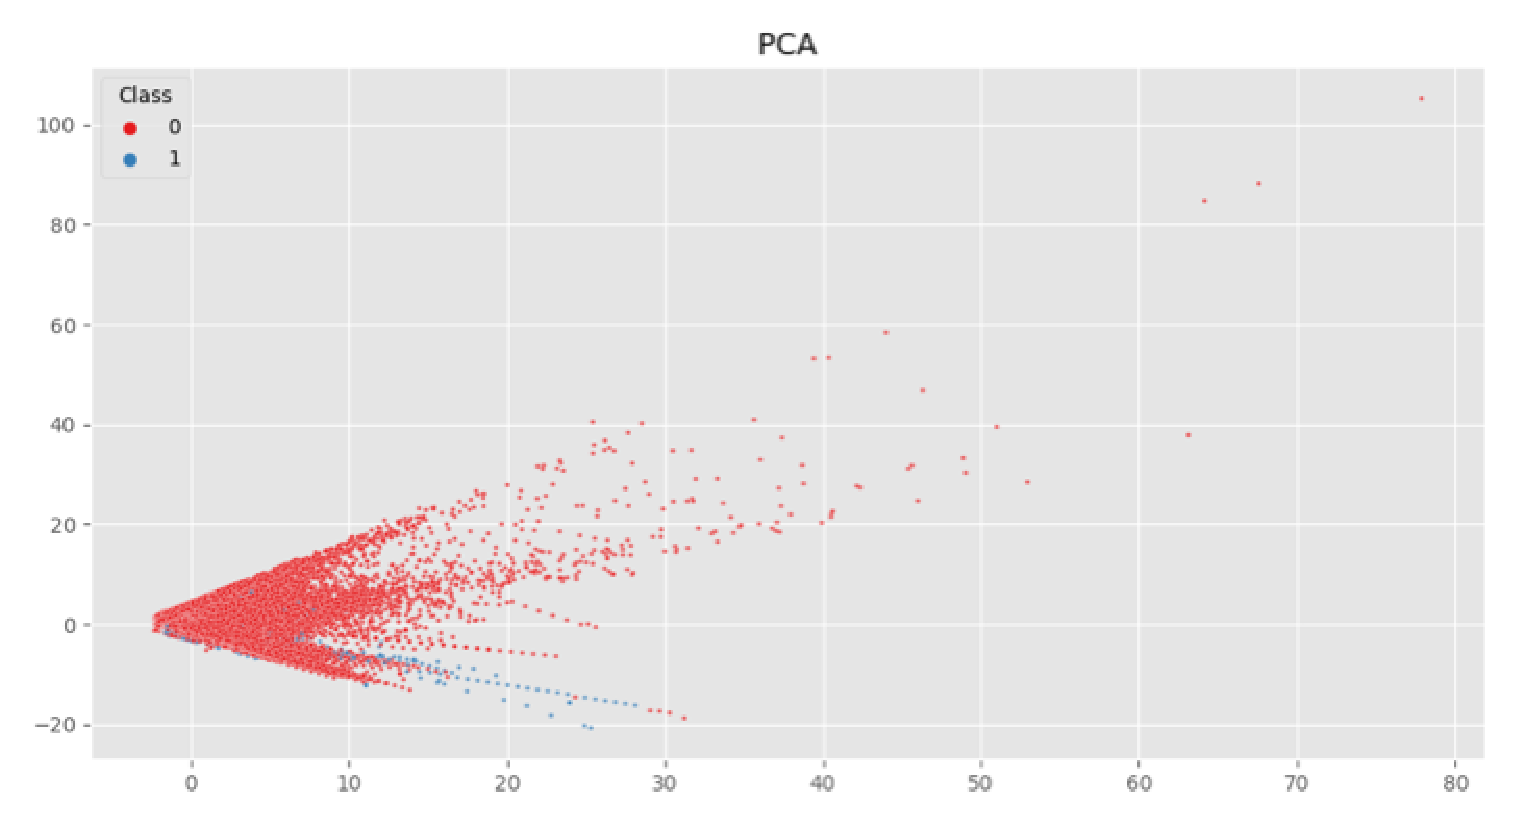
\includegraphics[scale=0.4]{pca.eps}
	%  \includegraphics[width=0.5\textwidth]{figures//OutAspect_target.eps}\\
	\caption{PCA}\label{fig:OutAspect-target}
	\end{figure}
	\end{center}
}{
	\begin{center}
		\begin{figure}
			\centering
			\selectcolormodel{rgb}
			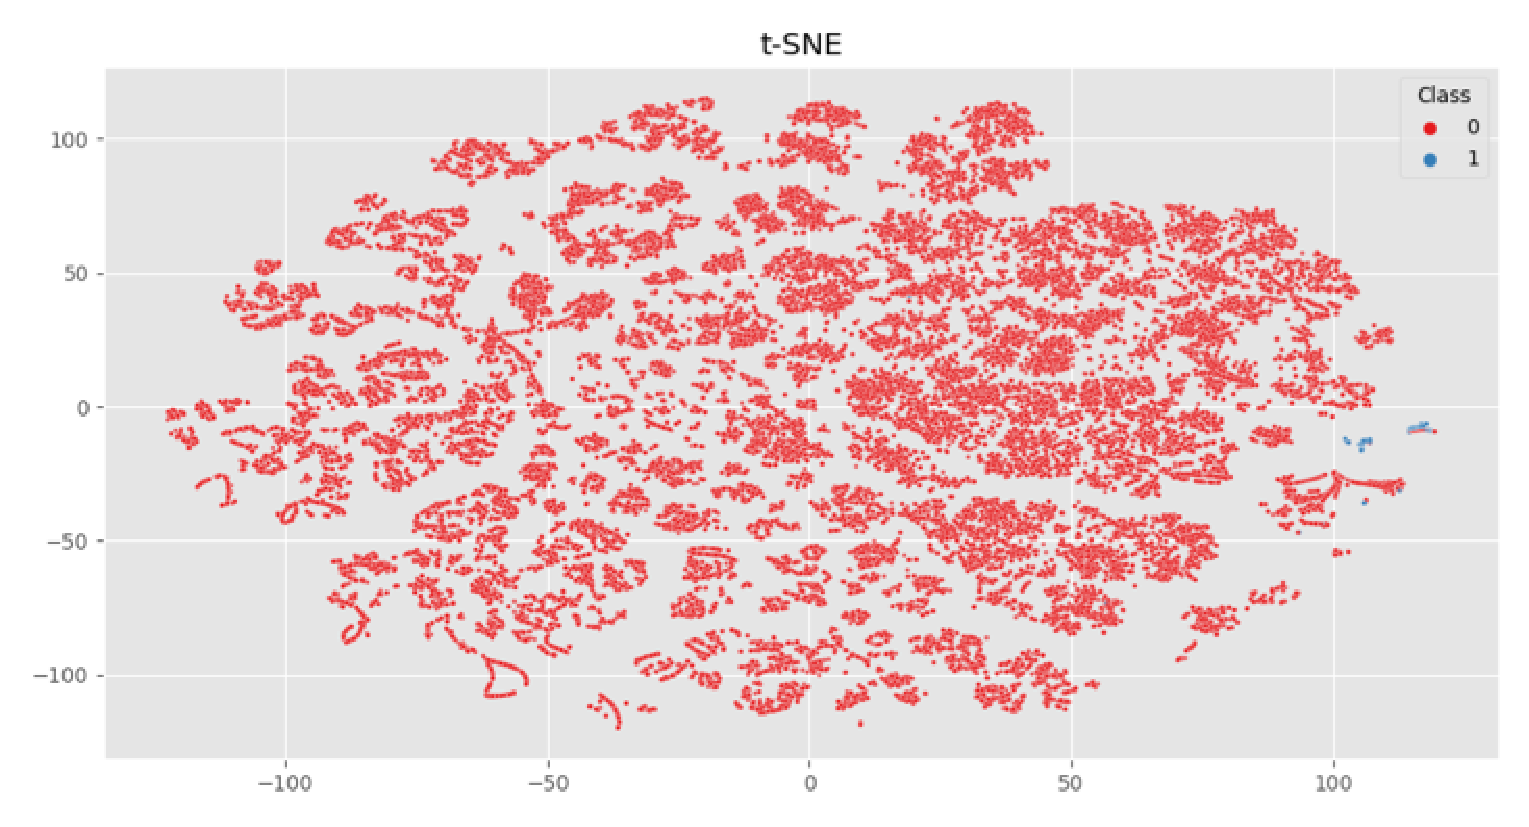
\includegraphics[scale=0.4]{tsne.eps}
			%  \includegraphics[width=0.5\textwidth]{figures//OutAspect_target.eps}\\
			\caption{t-SNE}\label{fig:OutAspect-target}
		\end{figure}
	\end{center}
}
	
\end{slide}
%%
%%=========================================================================================


==============
%%
\begin{slide}[toc=,bm=]{Data Preprocessing}
	\begin{itemize}
		\item
		Normalize the  \textcolor{orange} {Amount} and  \textcolor{orange} {Time columns} in the data.
	\end{itemize}
	\begin{itemize}
	\item
	Divide the  \textcolor{orange} {train} set and  \textcolor{orange} {test} set.
\end{itemize}
	\begin{itemize}
	\item
	30 Features- \textcolor{orange} {['Time','Amount','V1', 'V2', 'V3', 'V4', 'V5', 'V6', 'V7', 'V8', 'V9', 'V10', 'V11','V12', 'V13', 'V14', 'V15', 'V16', 'V17', 'V18', 'V19', 'V20', 'V21', 'V22', 'V23', 'V24', 'V25', 'V26', 'V27', 'V28']}.

\end{itemize}
\begin{center}
	\begin{tabular}{c| c c c c c }
	\toprule
	%\centering
	Data & \texttt{row_num}  & \texttt{Normal} & \texttt{Fraud} \\
	\midrule
	$train$
	&  {$227845$} &  {$227468$} &  {$377$} \\
	$test$
	&  {$57339$} &  {$56847$} &  {$115$} \\
	\bottomrule
\end{tabular}
\end{center}
\end{slide}
%%
%%==========================================================================================






\section{Unsupervised and Supervised Anomaly Detection Methods}

==============
%%
\begin{slide}[toc=,bm=]{Unsupervised - Isolation Forest}
	\begin{itemize}
		\item
		Isolation Forest(IF) is build based on decision trees. No pre-defined labels here. An unsupervised learning algorithm.\\
		1. Two quantitative properties of anomalous data points:Outliers are \textcolor{red} {few} and their features are very \textcolor{red} {different} from normal points.\\
		2. Not assume normal distribution and Detect outliers at a multi-dimensional level. \\
		3. Isolation Forest is computationally efficient: a low constant and a low memory requirement.	\\
		4. Parameters - \textbf{Number of estimators}, \textbf{Max samples}, \textbf{Contamination}, \textbf{Max features}
\end{itemize}

	\begin{figure}
		\centering
		\selectcolormodel{rgb}
		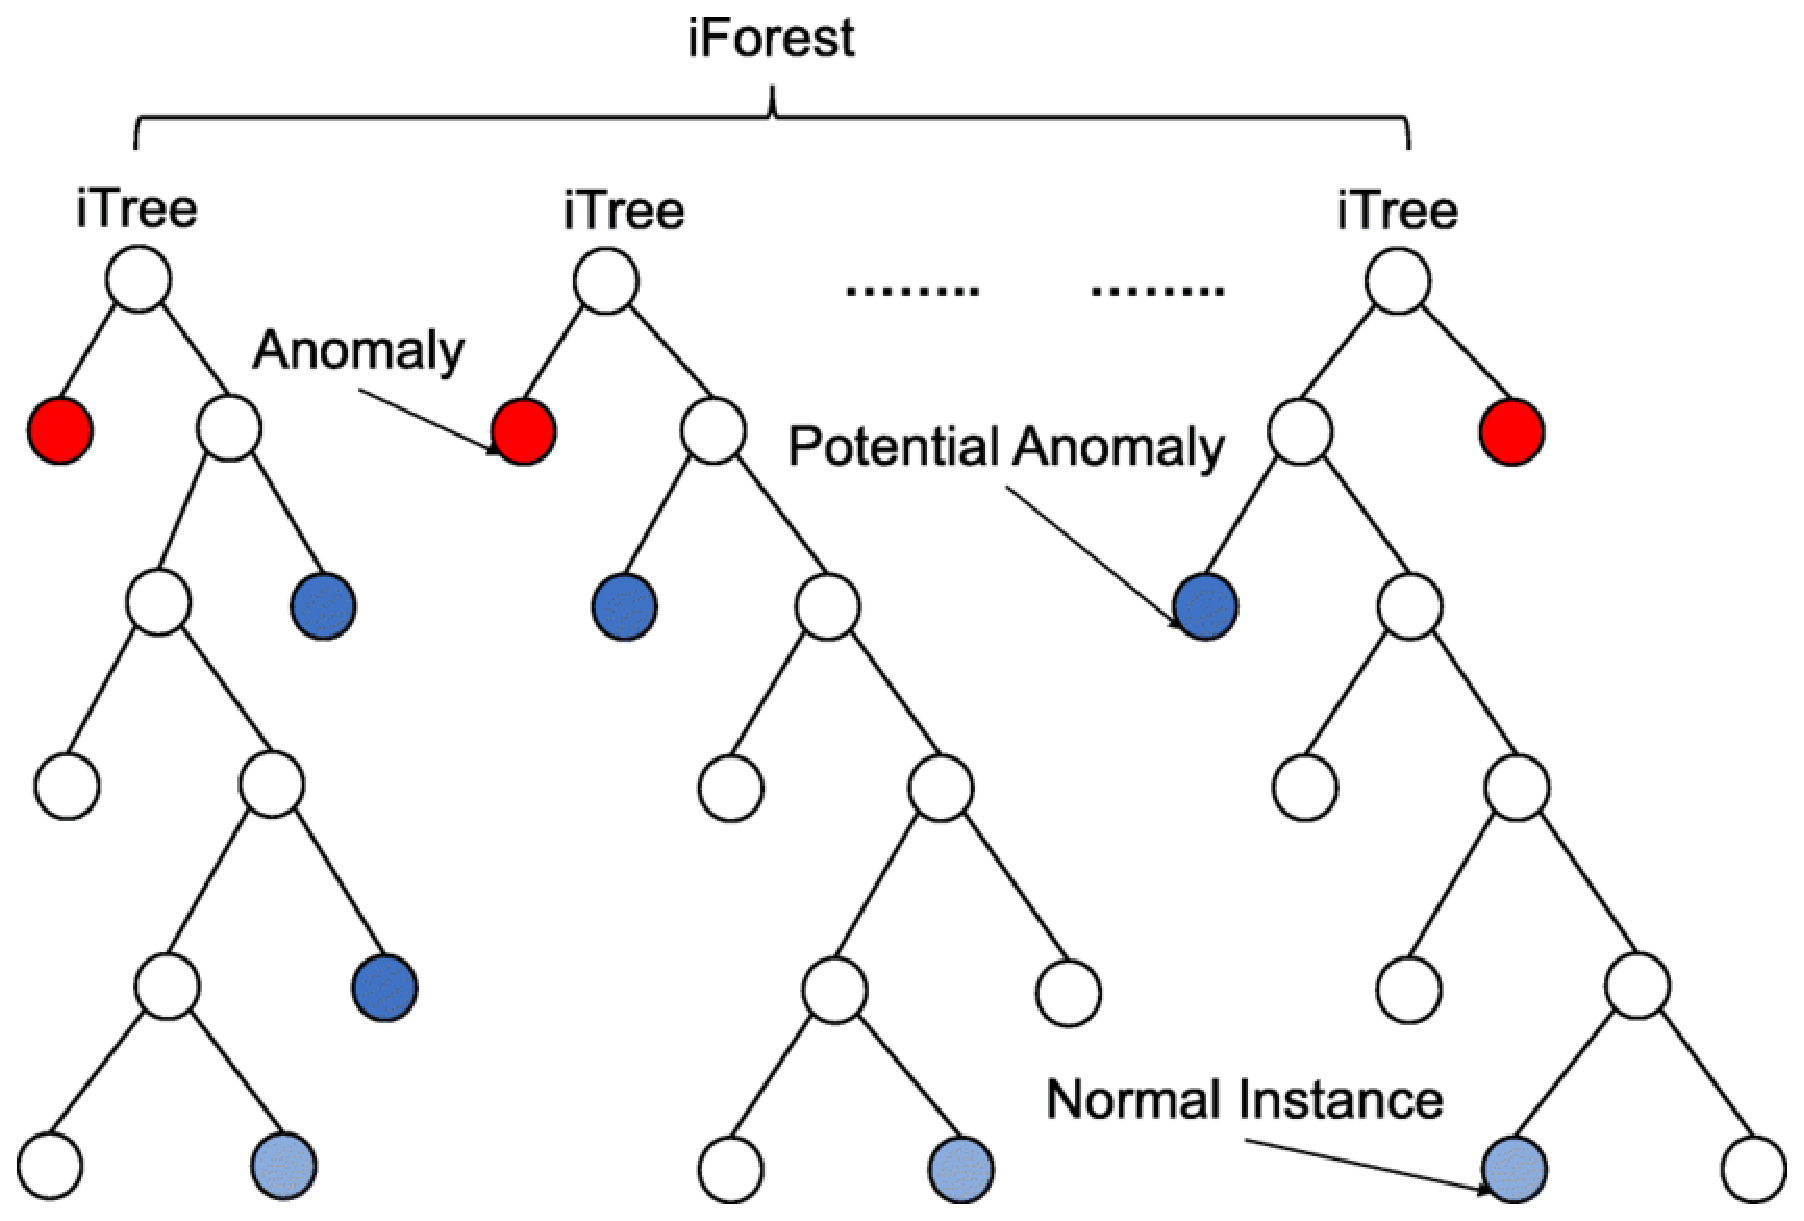
\includegraphics[scale=0.2]{iforest.eps}
		%  \includegraphics[width=0.5\textwidth]{figures//OutAspect_target.eps}\\
		% \caption{Aggregated time series}\label{fig:OutAspect-target}
	\end{figure}
\end{slide}
%%
%%==========================================================================================



\begin{slide}[toc=,bm=]{Unsupervised - DBSCAN}
	\begin{itemize}
	\item
	DBSCAN is a powerful density-based data clustering algorithm.\\
	1. DBSCAN algorithm separates the high-density regions of the data from the low-density areas.\\
	2. Detect outliers by identifying noise. \\
	3. Parameters - \textbf{Epsilon}, \textbf{minPoints}
\end{itemize}

\begin{figure}
	\centering
	\selectcolormodel{rgb}
	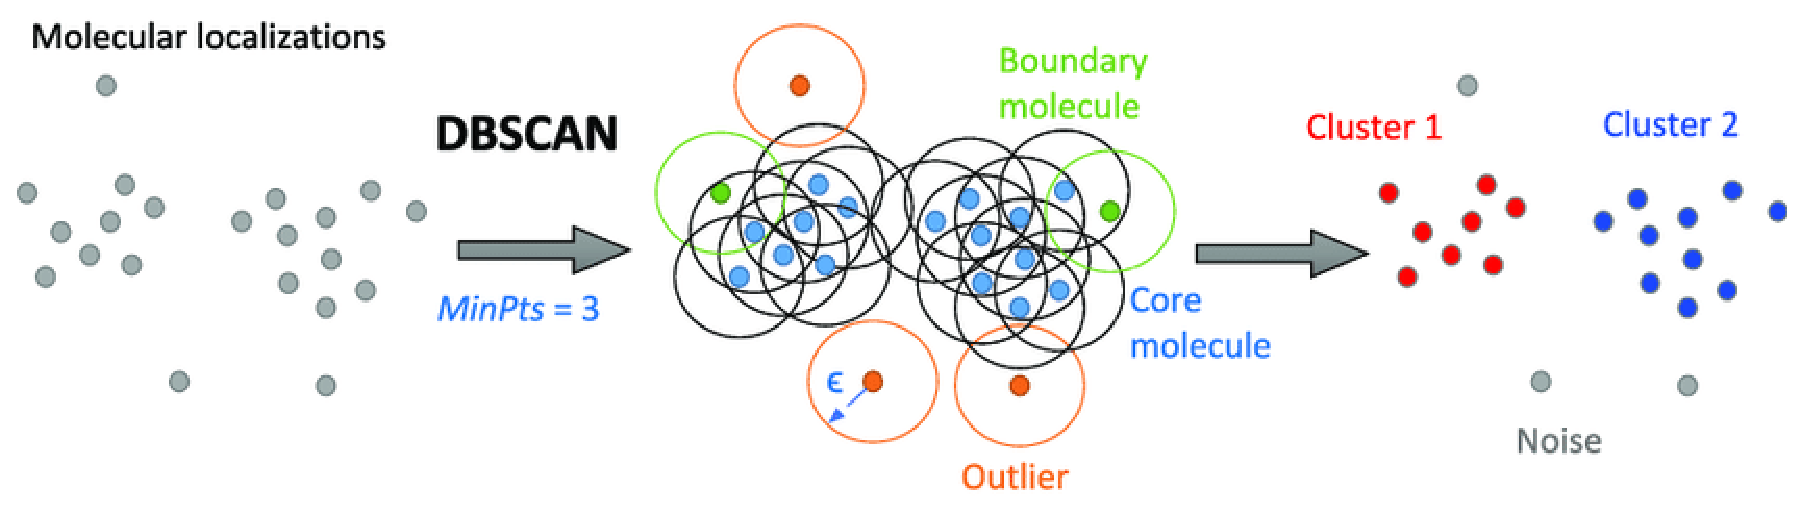
\includegraphics[scale=0.6]{dbscan.eps}
	%  \includegraphics[width=0.5\textwidth]{figures//OutAspect_target.eps}\\
	% \caption{Aggregated time series}\label{fig:OutAspect-target}
\end{figure}
\end{slide}
%%
%%==========================================================================================


%%==========================================================================================
%%
\begin{slide}[toc=,bm=]{Supervised - Random Forest}
		\begin{itemize}
		\item
	Random Forests perform classification by constructing multiple decision trees and combining their predictions.\\
	1. Constructing a decision tree from the train set.\\
	2. Prediction of test sets and feature importance exploration\\
	3. Parameters - \textbf{n_estimators}, \textbf{max_depth}, \textbf{min_samples_leaf}, \textbf{min_samples_split}
\end{itemize}

	\begin{figure}
		\centering
		\selectcolormodel{rgb}
		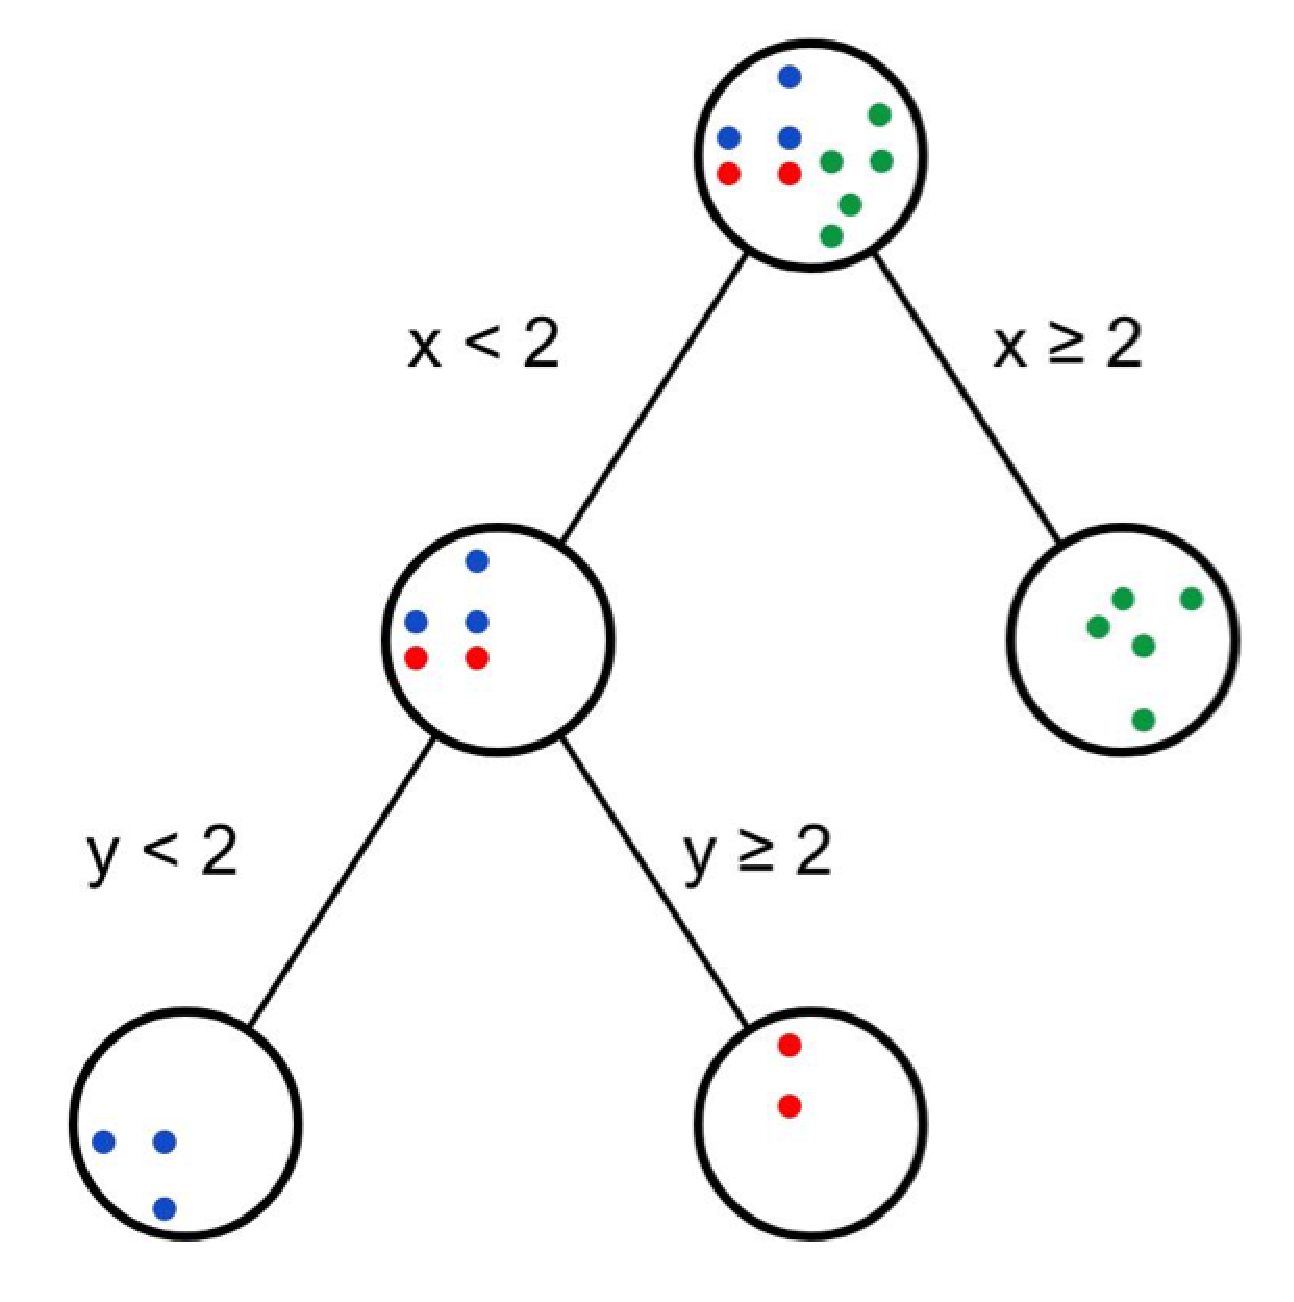
\includegraphics[scale=0.3]{rf.eps}
		%  \includegraphics[width=0.5\textwidth]{figures//OutAspect_target.eps}\\
	\end{figure}
\end{slide}
%%
%%==========================================================================================


%%==========================================================================================
%%
\begin{slide}[toc=,bm=]{Supervised - XGBoost}
		\begin{itemize}
		\item
		XGBoost (eXtreme Gradient Boosting) is a gradient boosting tree algorithm.\\
		1. The core principle is to combine multiple weak learners (decision trees) into one strong learner\\
		2. Decision trees are trained in an iterative manner to train new trees based on the residuals between the predictions   and the actual labels of all the previous trees in order to gradually reduce the error.\\
		3. Parameters - \textbf{n_estimators}, \textbf{max_depth}, \textbf{learning_rate}, \textbf{subsample}, \textbf{colsample_bytree}
	\end{itemize}
	
	\begin{figure}
		\centering
		\selectcolormodel{rgb}
		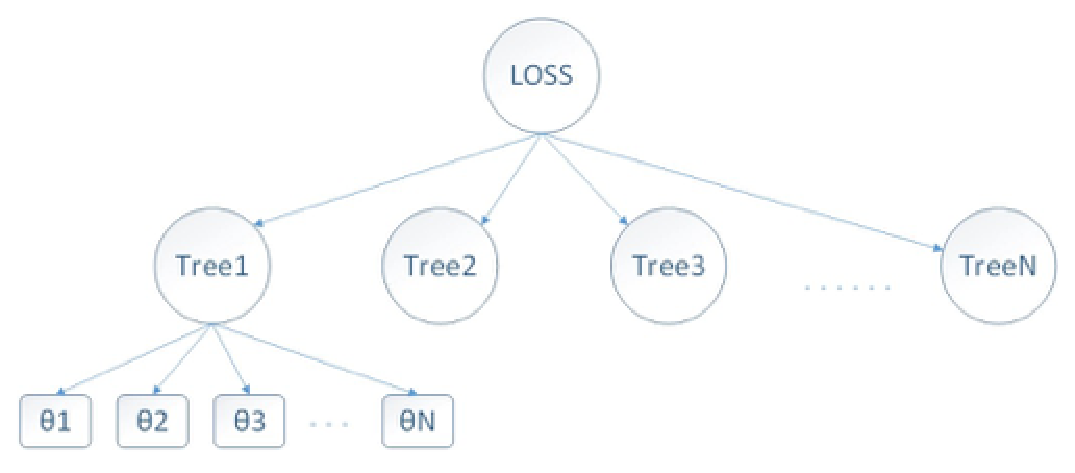
\includegraphics[scale=0.68]{xgb.eps}
		%  \includegraphics[width=0.5\textwidth]{figures//OutAspect_target.eps}\\

	\end{figure}


\end{slide}
%%
%%==========================================================================================


\section{Model Train and Result}


%%==========================================================================================
%%
\begin{slide}[toc=,bm=]{Model Train}
\begin{itemize}
	\item
	Each method has been subjected to a parameter network search and parameter tuning.Parameters not mentioned use default values.
\end{itemize}
\begin{center}
	\begin{tabular}{c| c c c c c }
		\toprule
		%\centering
		Method & \texttt{Type}  & \texttt{Train} & \texttt{Test}  \\
		\midrule
		$Isolation\ Forest$
		&  {$Unsupervised$} &  {$all\ data$} & {$all\ data$} \\
		$DBSCAN$
		&  {$Unsupervised$} &  {$all\ data$} & {$all\ data$} \\
		$Random\ Forest$
		&  {$Supervised$} &  {$train$} &  {$test$}  \\
		$XGBoost$
		&  {$Supervised$} &  {$train$} &  {$test$}  \\
		\bottomrule
	\end{tabular}
\end{center}
\begin{center}
	\begin{tabular}{c| c c c c c }
		\toprule
		%\centering
		Method & \texttt{ Parameters} \\
		\midrule
		$Isolation\ Forest$
		&   {$n\_estimators=1000,contamination=0.00172,max_features=1.0$} \\
		$DBSCAN$
		 &  {$eps=3.0, min\_samples=10$} \\
		$Random\ Forest$
		 &  {$n\_estimators=100$} \\
		$XGBoost$
		&  {$n\_estimators=100,learning\_rate=0.3,max\_depth=5$} \\
		\bottomrule
	\end{tabular}
\end{center}
\end{slide}
%%
%%==========================================================================================


%%==========================================================================================
%%
\begin{slide}[toc=,bm=]{Evaluation Method}

Use  \textbf{Accuracy}, \textbf{Precision}, \textbf{Recall}, and \textbf{F1} value to evaluate the model.
\begin{itemize}
\item
TP - True Fraud \quad TN -  True Normal\\
FP - False Normal \quad FN - False Fraud
\end{itemize}

	\begin{align}
	\text{Accuracy} = \frac{TP + TN}{TP + TN + FP + FN}
\end{align}
	\begin{align}
	\text{Precision} = \frac{TP}{TP + FP}
\end{align}
	\begin{align}
	\text{Recall} = \frac{TP}{TP + FN}
\end{align}
	\begin{align}
	\text{F1-score} = 2 \times \frac{\text{Precision} \times \text{Recall}}{\text{Precision} + \text{Recall}}
\end{align}

	
\end{slide}
%%==========================================================================================
\begin{slide}[toc=,bm=]{Result}
\begin{center}
	\begin{tabular}{c| c c c c c }
		\toprule
		%\centering
		Method & \texttt{Accuracy}  & \texttt{Precision} & \texttt{Recall}  & \texttt{F1}  & \texttt{Time(s)}\\
		\midrule
		$Isolation\ Forest$
		&  {$0.998$} &  {$0.314$} & {$0.313$} & {$0.314$}  & {$344$} \\
		$DBSCAN$
		&  {$0.946$} &  {$0.027$} & {$0.865$} & {$0.053$}  & {$182$} \\
		$Random\ Forest$
		&  {$0.999$} &  {$0.948$} & {$0.791$} & {$0.863$}  & {$314$} \\
		$XGBoost$
		&  {$0.999$} &  {$0.949$} & {$0.817$} & {$0.874$}  & {$56$} \\
		\bottomrule
	\end{tabular}
\end{center}
	\begin{figure}
		\centering
		\selectcolormodel{rgb}
		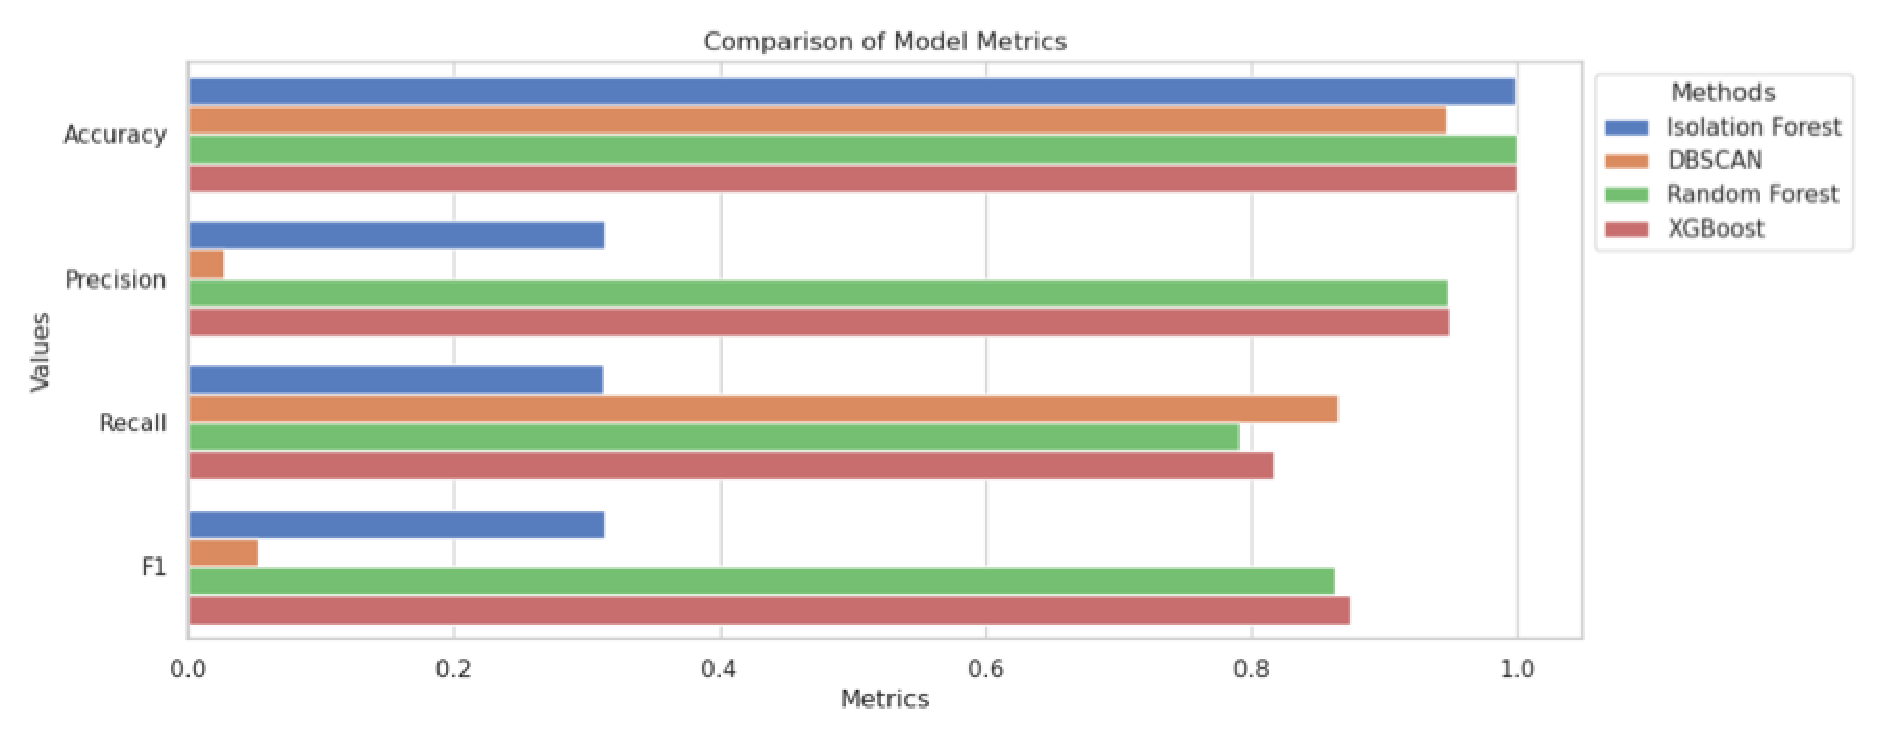
\includegraphics[scale=0.515]{result.eps}
		%  \includegraphics[width=0.5\textwidth]{figures//OutAspect_target.eps}\\
	\end{figure}
	
\end{slide}

\section{Conclusion}

%%==========================================================================================
%%
\begin{slide}[toc=,bm=]{Conclusion}
\begin{itemize}
\item
\smallskip
Supervised methods are superior to unsupervised methods.

\item
\smallskip
The performance of decision tree related methods is related to the number of decision trees and max depth.

\item
\smallskip
Based on correlation analysis and feature importance analysis, identifying credit card fraud is mainly related to features V4, V10, V11, V12, V14, and V17.

\end{itemize}
	\begin{figure}
	\centering
	\selectcolormodel{rgb}
	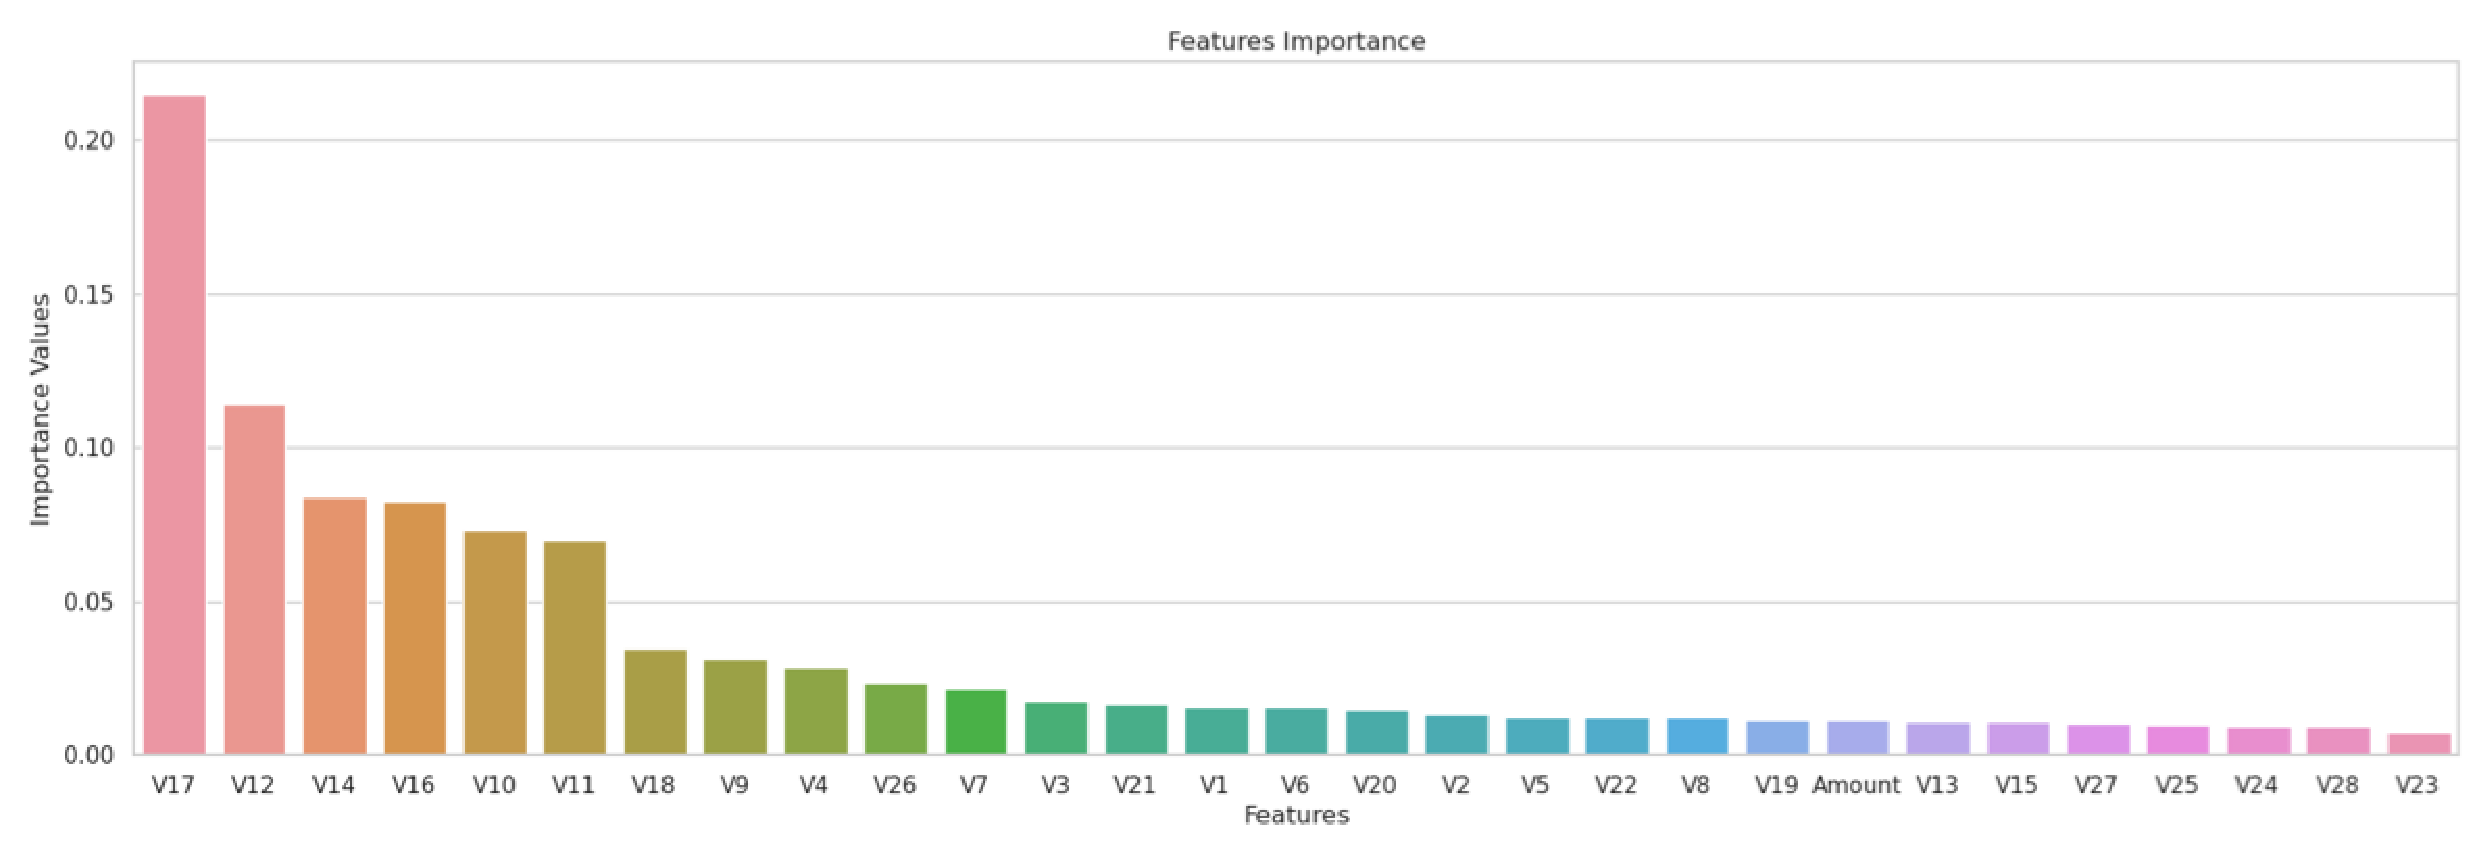
\includegraphics[scale=0.455]{fi.eps}
	%  \includegraphics[width=0.5\textwidth]{figures//OutAspect_target.eps}\\
\end{figure}
%%==========================================================================================
%%==========================================================================================

\end{slide}
%%
%%==========================================================================================


%%==========================================================================================
%
\begin{slide}[toc=,bm=]{Questions?}
\begin{center}
\begin{figure}
    \animategraphics[autoplay, loop, height=0.4\textheight]{5}{./graphics//gif//question//q_}{1}{30}
\end{figure}
\end{center}
\end{slide}
%%
%%==========================================================================================


%%==========================================================================================
% TODO: Contact Page
\begin{wideslide}[toc=,bm=]{Contact Information}
\centering
\vspace{\stretch{1}}
\twocolumn[
lcolwidth=0.35\linewidth,
rcolwidth=0.65\linewidth
]
{
% \centerline{\includegraphics[scale=.2]{tulip-logo.eps}}
}
{
\vspace{\stretch{1}}
Jiahong Lin\\
School of Economics and Management\\
Nanjing University of Science and Technology, China
\begin{description}
 \item[\textcolor{orange}{\faEnvelope}] \href{mailto:kksmi18@163.com}
 {\textsc{\footnotesize{kksmi18@163.com}}}


\end{description}
}
\vspace{\stretch{1}}
\end{wideslide}

\end{document}

\endinput
